\label{sec:brushing}
The tracking typically contains a few frames where the particle is not detected correctly due to being visually obstructed in some way. This causes to spikes in the data which complicates analysis. To make further theoretical analysis possible the data is corrected by removing such points manually. The basis for removal is a large discontinuity in the data, and many such points could be eliminated with algorithmic means. However in particular for $n_z$ it is very difficult to write an algorithm that catches all possible edge cases without having false positives. For example $n_z$ have peaks that make its derivative non continuous which means that a continuous derivative cannot be to exclude points. It's was found to be simpler to look at the analysis program and remove the points where the particle cannot be traced accurately due to noise. 

An example of data before and after correction can be seen in Figure \ref{fig:brushed} and all uncorrected data files of measurements used in this thesis are available at \url{http://goo.gl/jgzSXe}.

\begin{figure}[H]
\centering
\begin{subfigure}[3a]{0.40\textwidth}
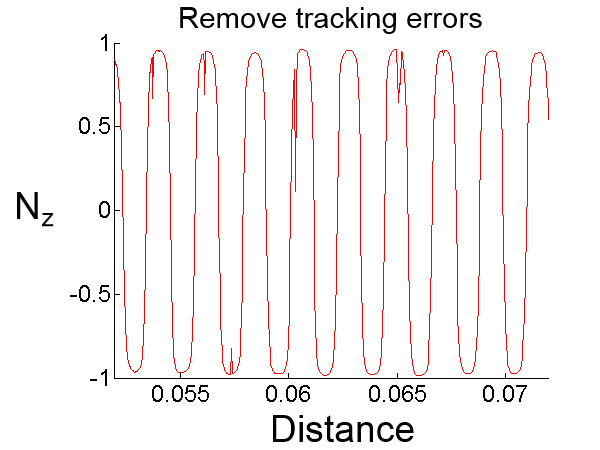
\includegraphics[width=\textwidth]{figures/method/Brushing1.png}
\caption{$n_x$ time series before correction.}\label{fig:prebrush}
\end{subfigure}\hspace{1em}%
\begin{subfigure}[3b]{0.40\textwidth}
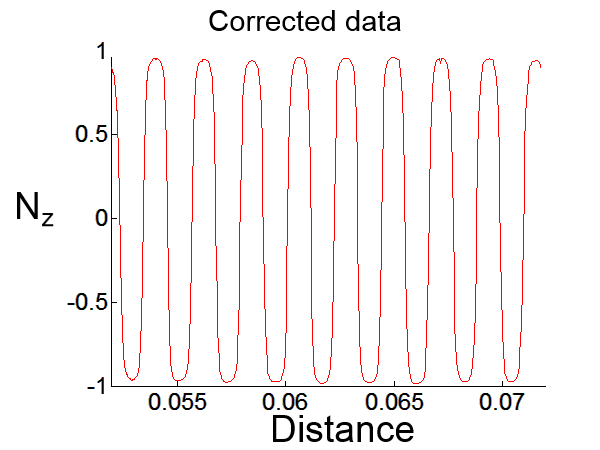
\includegraphics[width=\textwidth]{figures/method/Brushing2.png}
\caption{$n_x$ time series after correction.}\label{fig:postbrush}
\end{subfigure} \\
\caption{Shows screenshots from the software used to remove tracking errors for a time series of $n_z$ before and after removing points where a significant amount of noise disturbed the tracking.} \label{fig:brushed}
\end{figure}
